\documentclass[a4paper]{article}

% region packages
\usepackage{multicol}
\usepackage{calc}
\usepackage{ifthen}
\usepackage[landscape]{geometry}
\usepackage{hyperref}
\usepackage{blindtext}
\usepackage{xfrac}
\usepackage{amsmath}
\usepackage[portuguese]{babel}
\usepackage[raggedrightboxes]{ragged2e}
\usepackage{booktabs}
\usepackage{array}
\usepackage{tabularray}
\usepackage[none]{hyphenat}
\usepackage{titlesec}
\usepackage{fixmath}
\usepackage{tikz}
\usepackage{import}
\usepackage{xifthen}
\usepackage{pdfpages}
\usepackage{transparent}
\usepackage{amssymb}
% endregion
\geometry{top=1cm,left=1cm,right=1cm,bottom=1cm} % page margins
\pagestyle{empty} % Turn off header and footer
\setcounter{secnumdepth}{0} % Don't print section numbers
% region Redefine section commands to use less space
\titlespacing{\section}{0pt}{0pt}{0pt}
\titlespacing{\subsection}{0pt}{0pt}{0pt}
\titlespacing{\subsubsection}{0pt}{0pt}{0pt}
% endregion

\setlength{\parindent}{0pt}
\setlength{\parskip}{0pt plus 0.5ex}
\graphicspath{{./imgs/}}
\newcommand{\incfig}[1]{% todo not working lol
  \def\svgwidth{\columnwidth}
  \import{./figures/}{#1.pdf_tex}
}


% -----------------------------------------------------------------------

\begin{document}
\raggedright
\begin{multicols}{3}
% These lengths are set only within the two main columns
%\setlength{\columnseprule}{0.25pt}
\setlength{\premulticols}{1pt}
\setlength{\postmulticols}{1pt}
\setlength{\multicolsep}{1pt}
\setlength{\columnsep}{2pt}

\begin{center}
  \Large{\textbf{Estatística Computacional}} \\
  \small{Plancha; 105289; CDB2} \\
  \small{Versão 0.1}
\end{center}

\section{Teoria de Probabilidades}

\begin{tblr}{X c X[2]}\SetRow{m}
  Esperiência aleatória & & Processo de observação de fenómenos aleatórios \\
  Fenómenos aleatórios & & Acontecimentos não determináveis \textit{a priori} \\ \SetRow{m} 
  Espaço de resultados & $\Omega$ & Conjunto de todos os resultados possíveis \\ \SetRow{m}
  Acontecimentos & $A, B, C$ & Conjunto de possíveis resultados de uma experiência  \\ \SetRow{m}
  Resultado da experiência aleatória & $\omega$ & $A$ realizou-se se $\omega \in A$ 
\end{tblr}

\subsection{Álgebra dos acontecimentos}
\subsubsection{União}
$$A \cup B = \{ \omega : \omega \in A \lor \omega \in B \}$$
\subsubsection{Intersecção}
$$A \cap B = \{ \omega: \omega \in A \land \omega \in B \}$$
\subsubsection{Diferença}
$$A - B = A \setminus B = \{ \omega: \omega \in A \land \omega \notin B \}$$
$$\Omega - B = \overline{B} = \{ \omega: \omega \in \Omega \land \omega \notin B \}$$
\subsubsection{Propriedades}
\begin{tblr}{l r}
  Comutativa & {$A \cup B = B \cup A$ \\ $A \cap B = B \cap A$} \\
  Associativa & {$A \cup (B \cup C) = (A \cup B) \cup C$ \\ $A \cap (B \cap C) = (A \cap B) \cap C$} \\
  Distributiva & {$A \cup (B \cap C) = (A \cup B) \cap (A \cup C)$ \\ $A \cap (B \cup C) = (A \cap B) \cup (A \cap C)$} \\
  Idempotência & {$A \cup A = A$ \\ $A \cap A = A$} \\
  Lei do Complemento & {$A \cup \overline{A} = \Omega$ \\ $A \cap \overline{A} = \emptyset$}
\end{tblr} %column break
\subsubsection{Probabilidades (Cont)}
\begin{tblr}{l r}

  Elemento Neutro & {$A \cup \emptyset = A$ \\ $A \cap \Omega = A$} \\
  Elemento Absorvente & {$A \cup A = A$ \\ $A \cap \emptyset = \emptyset$} \\
  Leis de Morgan & {$\overline{A \cup B} = \overline{A} \cap \overline{B}$ \\ $\overline{A \cap B} = \overline{A} \cup \overline{B}$}
\end{tblr}

\subsection{Probabilidades}
\textit{a priori}:
$$P[A] = \frac{n_A}{N}$$
\textit{a posteriori}:
$$f_A = \frac{N_A}{N}$$
$$P[A] = \lim_{N \to \infty} f_A$$
\subsubsection{Definições}
\begin{tblr}{l r}
  $\overline{A}$ & $\Omega - A$ \\
  $P[A]$ & Probabilidade de $A$ \\
  $n_A$ & Número de resultados favoráveis a $A$ \\
  $N$ & Número de resultados possíveis \\
  $f_A$ & Frequência relativa de $A$ \\
  $N_A$ & Número de vezes que A se verificou \\
  $P[A \mid B]$ & Probabilidade de $A$ dado que $B$ se verificou \\
\end{tblr}
\subsubsection{Axiomas}
$$\forall A \subseteq \Omega: 0 \leq P[A] \leq 1$$
$$P[\Omega] = 1$$
Independência/Acontecimentos mutualmente exclusivos:
$$\forall A, B \subseteq \Omega \ni A \cap B = \emptyset: P[A \cup B] = P[A] + P[B]$$
\subsubsection{Teoremas}
\begin{align*}
  &P[\overline{A}] = 1 - P[A] \\
  &P[\emptyset] = 0 \\
  &P[B-A] = P[B] - P[A \cap B] \\
  &P[A \cup B] = P[A] + P[B] - P[A \cap B] \\
  & P[A \cup B \cup C] = P[A] + P[B] + P[C] \\ 
  &\qquad - P[A \cap B] - P[A \cap C] - P[B \cap C] \\ 
  &\qquad + P[A \cap B \cap C] \\
  &P[A \cup B] \leq P[A] + P[B] \\
  &P[A \mid B] = \frac{P[A \cap B]}{P[B]} & \text{se} \; P[B] > 0 \\
  &P[A \mid B] = 0 & \text{se} \; P[B] = 0
\end{align*}
Para acontecimentos independentes:
\begin{align*}
& P[A \cap B] = P[A] \cdot P[B] \\
& P[A \mid B] = P[A]
\end{align*}
\subsubsection{$\mathbold{n}$ partições:} 
$$\cup_{i=1}^n A_i = \Omega$$
$$A_i \cap A_j = \emptyset$$
$$P[A_i] > 0$$
Teorema da Probabilidade total:
$$\forall B \subseteq \Omega: P[B] = \sum_{i=1}^n P[A_i \cap B]$$
$$\forall B \subseteq \Omega: P[B] = \sum_{i=1}^n P[A_i \mid B] \cdot P[B]$$
Fórmula de Bayes:
$$P[A_j \mid B] = \frac{P[A_j] \cdot P[B \mid A_j]}{\sum_{i=1}^n P[A_i] \cdot P[B \mid A_i]}$$
\pagebreak
\subsection{Variáveis aleatórias}
$$P[X = x] = P[A] = P[{\omega \in \Omega: X(\omega) = x}]$$
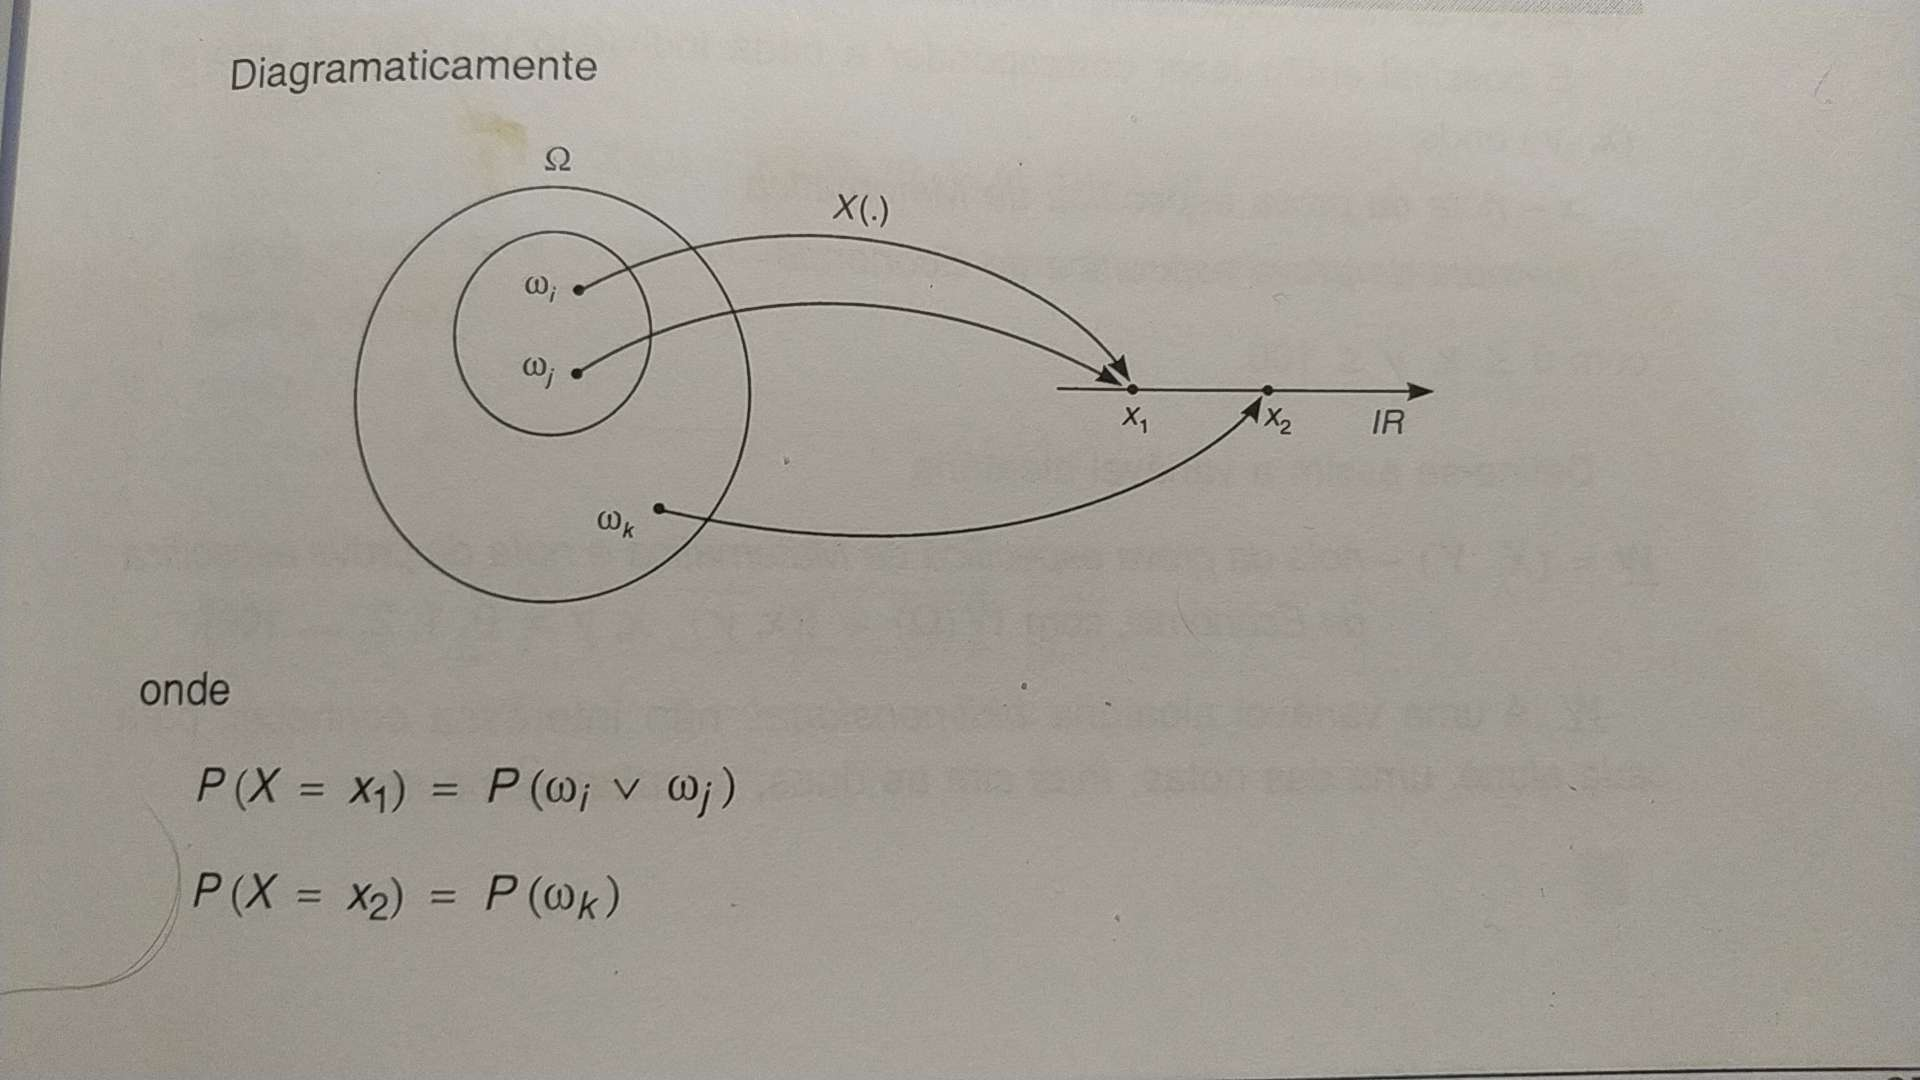
\includegraphics[width=\columnwidth]{variaveisAleatorias.jpg} %TODO mudar para tex (geogebra?)
\begin{tblr}{X l X[2]}\SetRow{m}
  Variável aleatória & $X(\omega)\; \text{ou}\; X$ & Função que cada acontecimento $\omega$ associa um valor real $x = X(\omega)$ \\\SetRow{m}
  CD de uma Variável aleatória & $X(\Omega)$ & 
\end{tblr}
\subsubsection{Função (massa) de probabilidade}
X é discreto
\begin{align*}
  &f(x) = P[X = x] \\
  &0 \leq f(x) \leq 1 \\
  &\sum_{i=1}^n f(x_i) = 1 & \text{caso } n {\text{ finito}} \\
  &\sum_{i=1}^{\infty} f(x_i) = 1 & \text{caso } n {\text{ infinito}} \\
\end{align*}
\subsubsection{Função densidade de probabilidade}
X é contínuo, e é comum a função ser parametrizada (p.e. $f(x;\mu ,\sigma ^{2})$), dependendo da distribuição de X
\begin{align*}
  &f(x) = \frac {d}{dx}F(x) \\
  &0 \leq f(x) \leq 1 \\
  &\int_{-\infty}^{\infty} f(x) dx = 1 \\
  &P[X = x] = 0 \; f(x) \neq 0
\end{align*}
\subsubsection{Função de distribuição (acomuldada) (f.d.p.)}
A função é apenas crescente
\begin{align*}
  &F(x) = P[X \leq x] \\
  &0 \leq F(x) \leq 1 \\
  &\forall x_2 > x_1: \\
    &\qquad F(x_2) \geq F(x_1) \\ 
    &\qquad \land F(x_2) - F(x_1) = P[x_1 < X \leq x_2] \\
  &\lim_{x \to -\infty} F(x) = 0 \\ 
  &\lim_{x \to \infty} F(x) = 1 \\
  &P[x_1 < X \leq x_2] = F(x_2) - F(x_1)
\end{align*}
Se $X$ for contínua:
\begin{align*}
  &F(x) = P[X \leq x] = \int_{-\infty}^x f(u) du \\
  &P[x_1 < X \leq x_2] = \int_{x_1}^{x_2} f(u) du
\end{align*}
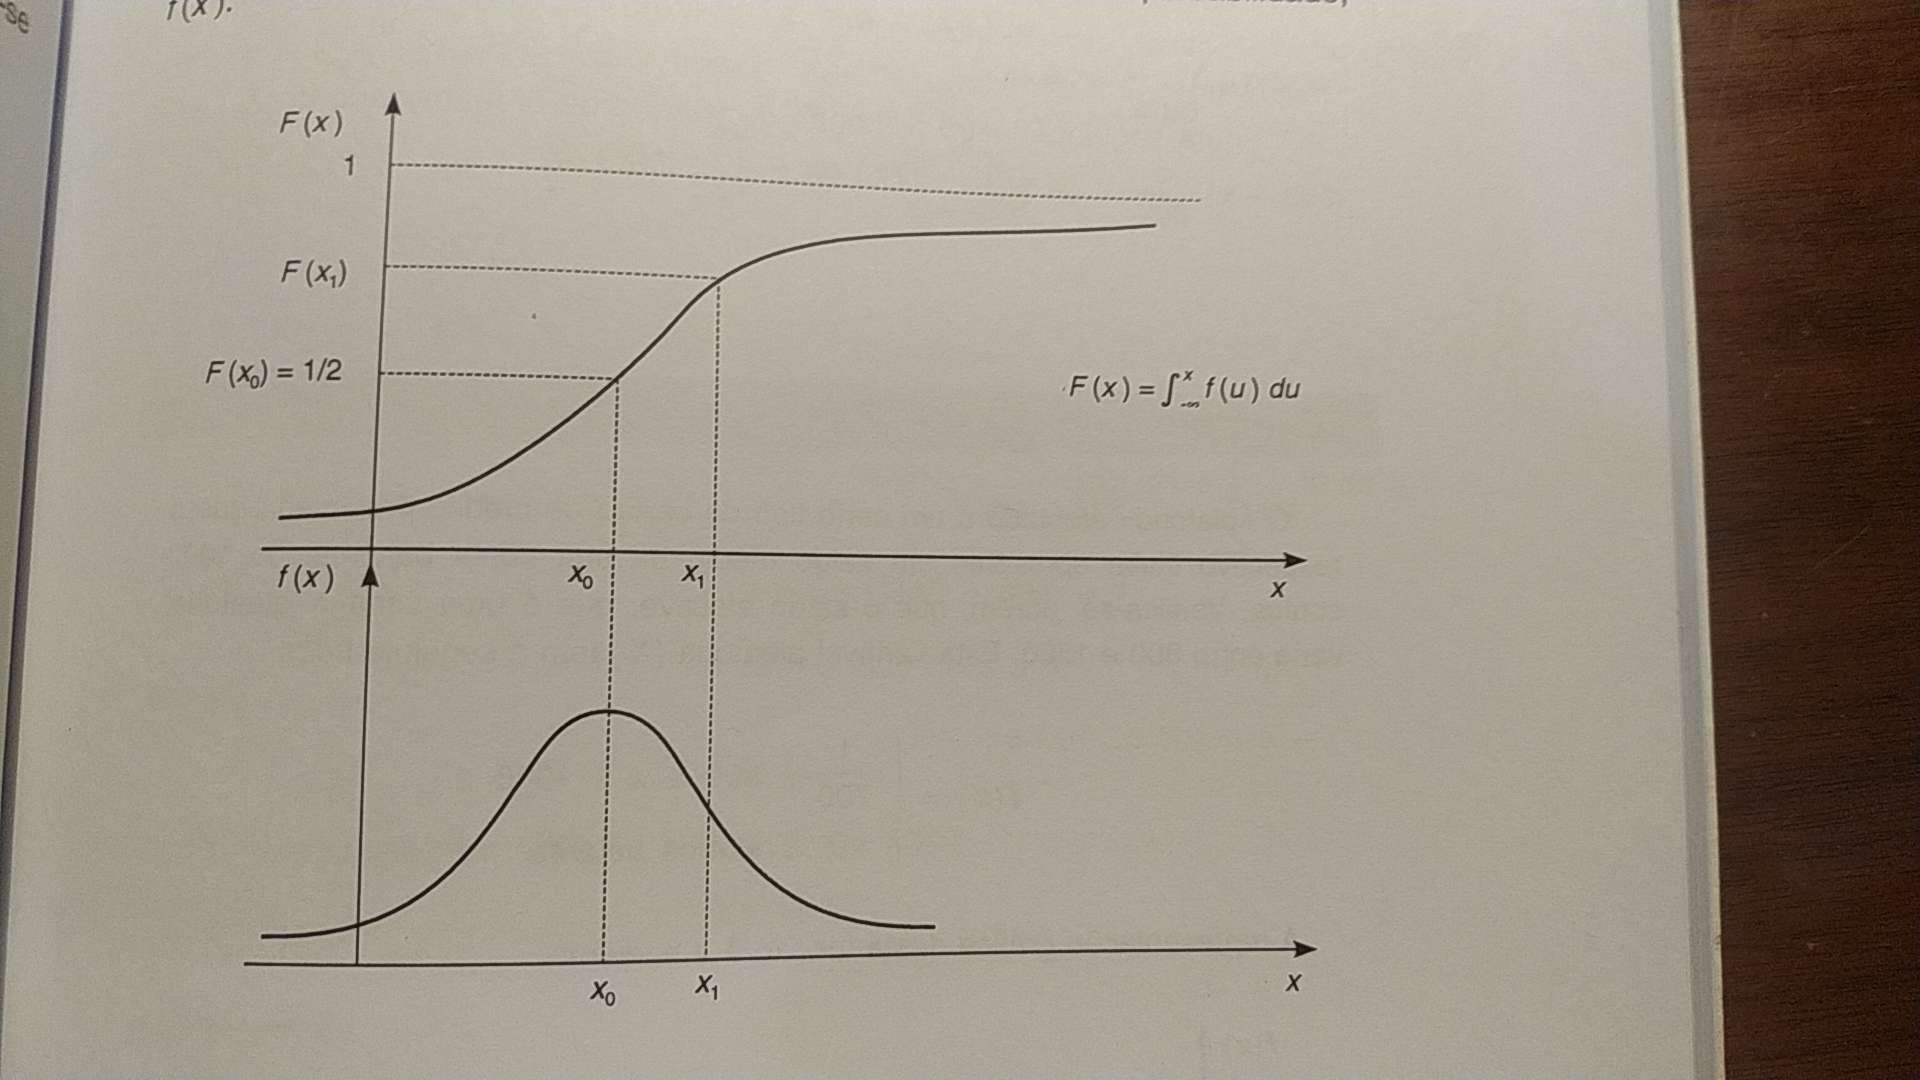
\includegraphics[width=\columnwidth]{fda.jpg} %TODO mudar para tex (geogebra?)
\subsection{Função de probabilidade conjunta}
Se discretas
\begin{align*}
  &f(x, y) = P[X = x, Y = y] = P[X = x \cap Y = y]\\
  &0 \leq f(x, y) \leq 1 \\
  &\sum_{i=1}^n \sum_{j=1}^n f(x_i, y_j) = 1 \\
  &F(x, y) = P[X \leq x, Y \leq y] = \sum_{x_i \leq x} \sum_{y_j \leq y} f(x_i, y_j) \\
  &\lim_{x \to -\infty \land y \to -\infty} F(x, y) = 0 \\
  &\lim_{x \to \infty \land y \to \infty} F(x, y) = 1 \\
  &\forall \lambda \in \mathbb{R}: \\
    &\qquad \lim_{x \to -\infty } F(x, \lambda) = \lim_{y \to -\infty } F(\lambda, y) = 0 \\
  &\forall x_2 > x_1 \land y_2 > y_1: F(x_2, y_2) \geq F(x_1, y_1)
\end{align*}
Se contínuas

\begin{align*}
  &f(x, y) = \frac{\partial^2 F(x, y)}{\partial x \partial y} \\
  &F(x, y) = \int_{-\infty}^x \int_{-\infty}^y f(u, v) dv du \\
\end{align*}

\subsection{Parâmetros de v.a.s}
\subsection{Valor esperado}
O valor esperado de $X$ é igual à média de $X$.
$$E[X] = \mu_X = \mu$$
Se $X$ for discreta:
$$E[X] = \sum_i x_i \cdot f(x_i)$$
Se $X$ for contínua:
$$E[X] = \int x \cdot f(x) dx$$
\subsubsection{Propriedades}
\begin{align*}
  &E[\lambda] = \lambda \\
  &E[\lambda X] = \lambda E[X] \\
  &E[X \pm Y] = E[X] \pm E[Y] \\
  &E[X Y] = E[X] E[Y] & \text{se } X \text{ e } Y \text{ forem independentes} \\
  &E[g(X)] = \sum_i g(x_i) \cdot f(x_i) \iff \text{se } X \text{ for discreta} \\
  &E[g(X)] = \int g(x) \cdot f(x) dx \iff \text{se } X \text{ for contínua} \\
  &E[X^2] = \sum_i x_i^2 \cdot f(x_i) \iff \text{se } X \text{ for discreta}
\end{align*}
%TODO finish + organize Variancia 
% aqui está apenas o importante para o teste
\subsection{Variância}
\begin{align*}
  &VAR(X) = \sigma^2_X = \sigma^2 \\
  &VAR(X) = E[(X - E[X])^2] \\
  &VAR(X) = E[X^2] - E[X]^2 \\
  &VAR(X) = E[X^2] - \mu^2 \\
  &VAR(X) = \sum_i (x_i - \mu)^2 \cdot f(x_i) \iff \text{se } X \text{ for discreta} \\
  &VAR(X) = \int (x - E[X])^2 \cdot f(x) dx \iff \text{se } X \text{ for contínua} \\
  &VAR(\lambda) = 0 \\
  &VAR(\lambda X) = \lambda^2 VAR(X) \\
  &VAR(X \pm Y) = VAR(X) + VAR(Y) \pm 2 cov(X, Y) \\
  &\sigma = \sqrt{VAR(X)} = \sqrt{\sigma^2} \\
  &Cov(X, Y) = E[(X - \mu_X)(Y - \mu_Y)] \\
  &Cov(X, Y) = E[X \cdot Y] - \mu_x \cdot \mu_y \\
  &Cov(X, Y) = 0 \iff X \text{ e } Y \text{ são independentes} \\
\end{align*}
% falta correlação linear mas n é preciso para este teste me thinks
% also falta momentos mas reza
% also desigualdades
$$W = \frac{X - \mu_X}{\sigma}$$,
$E(W) = 0$ e $VAR(W) = 1$.



\section{temp}
\blinddocument
\end{multicols}
\end{document}
